\section{Marginal value of public funds}

Evaluating a tax reform requires weighing the private welfare gained or lost by affected taxpayers against the net change in government revenue once behavioral adjustments are accounted for. This section evaluates a proposed reduction of Chile's top marginal personal income tax rate from $\tau_0 = 40\%$ to $\tau_1 = 35\%$. Part~(i) derives from first principles the mechanical revenue effect, the behavioral revenue offset under a Pareto upper tail and isoelastic utility, and the resulting Marginal Value of Public Funds (MVPF). Part~(ii) calibrates the model by combining the Chilean upper-tail Pareto parameters estimated in Problem Set~1 with top-bracket bunching elasticities recovered from the administrative binned records (\texttt{synthetic\_bunch\_counts.csv}). Part~(iii) synthesizes the empirical results into a self-contained policy brief detailing the underlying assumptions, caveats, and final recommendation.

\subsection*{(i) Mechanical effect, behavioral response, and the MVPF}

To isolate the fiscal and welfare effects of changing the top tax rate, we first specify the piecewise-linear tax schedule and the distribution of taxpayers in the upper bracket. Suppose the top tax bracket begins at threshold $z^* > 0$ and taxes every peso of income strictly above $z^*$ at marginal rate $\tau \in (0, 1)$, while $T_0(z^*)$ denotes the cumulative tax liability on income up to $z^*$ (which depends solely on lower-bracket rates and thresholds). A taxpayer in the top bracket ($z \ge z^*$) faces total tax liability
\begin{equation}
T(z; \tau) = T_0(z^*) + \tau(z - z^*).
\label{eq:p3_tax_func}
\end{equation}
Normalize the total taxpayer population to unit mass, with continuously differentiable cumulative distribution function $F(z)$ and probability density $f(z) = F'(z)$. The fraction of taxpayers located in the top bracket is
\begin{equation}
\int_{z^*}^\infty f(z)\,dz = 1 - F(z^*),
\label{eq:p3_top_mass}
\end{equation}
and the conditional mean taxable income among top-bracket taxpayers is
\begin{equation}
\bar{y} \equiv \mathbb{E}[z \mid z \ge z^*] = \frac{\int_{z^*}^\infty z\,f(z)\,dz}{1 - F(z^*)}
\qquad\Longleftrightarrow\qquad
\int_{z^*}^\infty z\,f(z)\,dz = \big(1 - F(z^*)\big)\bar{y}.
\label{eq:p3_ybar_def}
\end{equation}

\paragraph{Derivation of the mechanical effect $\Delta R^M$.}
We begin by computing the direct fiscal impact of an infinitesimal change $d\tau$ in the top marginal rate under frozen behavior—that is, holding every taxpayer's declared income $z$ fixed at its pre-reform level.\marginnote{For a rate cut from $\tau_0 = 0.40$ to $\tau_1 = 0.35$, $d\tau = \tau_1 - \tau_0 = -0.05 < 0$, so $\Delta R^M < 0$ measures the static revenue loss before accounting for behavioral expansion of the tax base.} Differentiating~\eqref{eq:p3_tax_func} with respect to $\tau$ at fixed $z \ge z^*$ yields the individual mechanical tax change
\begin{equation}
\Delta T^M(z) = \frac{\partial T(z; \tau)}{\partial \tau}\,d\tau = (z - z^*)\,d\tau,
\end{equation}
whereas $\Delta T^M(z) = 0$ for inframarginal taxpayers below $z^*$. Integrating $\Delta T^M(z)$ across the taxpayer distribution and substituting~\eqref{eq:p3_top_mass}--\eqref{eq:p3_ybar_def} yields
\begin{align}
\Delta R^M &= \int_{z^*}^\infty (z - z^*)\,d\tau\,f(z)\,dz \nonumber\\
&= d\tau \left[ \int_{z^*}^\infty z\,f(z)\,dz - z^* \int_{z^*}^\infty f(z)\,dz \right] \nonumber\\
&= d\tau \Big[ \big(1 - F(z^*)\big)\bar{y} - z^*\big(1 - F(z^*)\big) \Big] \nonumber\\
&= d\tau\,\big(1 - F(z^*)\big)(\bar{y} - z^*).
\label{eq:p3_mech}
\end{align}
Equation~\eqref{eq:p3_mech} shows that the static revenue effect equals the rate change $d\tau$ multiplied by the aggregate top-bracket tax base above the cutoff, $\big(1 - F(z^*)\big)(\bar{y} - z^*)$.

\paragraph{Derivation of the behavioral effect $\Delta R^B$.}
In practice, taxpayers adjust their reported income when marginal tax incentives change, generating a fiscal externality on government revenue. To express this behavioral offset in terms of observable sufficient statistics, consider the quasilinear, isoelastic preferences $u(c,z) = c - \frac{n^{-1/\epsilon}}{1+1/\epsilon}z^{1+1/\epsilon}$ analyzed in Sections~1 and~2. An agent locating in the interior of the top bracket ($z > z^*$) maximizes $(1-\tau)(z - z^*) + z^* - T_0(z^*) - \frac{n^{-1/\epsilon}}{1+1/\epsilon}z^{1+1/\epsilon}$, which yields the taxable-income supply function $z(n; \tau) = n(1-\tau)^\epsilon$. Consequently, the elasticity of taxable income (ETI) with respect to the net-of-tax rate $(1-\tau)$ is constant and equal to $\epsilon$:
\begin{equation}
\epsilon \equiv \frac{\partial \ln z(n; \tau)}{\partial \ln(1-\tau)} = \frac{1-\tau}{z}\,\frac{\partial z}{\partial(1-\tau)}.
\label{eq:p3_eti_def}
\end{equation}
Because $d(1-\tau) = -d\tau$, applying the chain rule to~\eqref{eq:p3_eti_def} pins down each top-bracket taxpayer's income adjustment $dz$ in response to $d\tau$:
\begin{equation}
dz = \frac{\partial z}{\partial(1-\tau)}\,d(1-\tau) = \left(\epsilon\,\frac{z}{1-\tau}\right)(-d\tau) = -\frac{\epsilon}{1-\tau}\,z\,d\tau.
\label{eq:p3_dz}
\end{equation}
Since every marginal peso above $z^*$ is taxed at rate $\tau$, an individual income response $dz$ alters tax collections by $\tau\,dz = -\frac{\tau}{1-\tau}\epsilon\,z\,d\tau$.\footnote{By Leibniz's integral rule, marginal taxpayers crossing the kink $z^*$ as $\tau$ varies by $d\tau$ generate only a second-order revenue effect $\mathcal{O}((d\tau)^2)$ because the tax schedule $T(z;\tau)$ is continuous at $z = z^*$.} Aggregating this behavioral revenue change over all top-bracket taxpayers and using~\eqref{eq:p3_ybar_def} gives
\begin{equation}
\Delta R^B = \int_{z^*}^\infty \tau\,dz\,f(z)\,dz
= -\frac{\tau}{1-\tau}\,\epsilon\,d\tau \int_{z^*}^\infty z\,f(z)\,dz
= -\frac{\tau}{1-\tau}\,\epsilon\,d\tau\,\big(1 - F(z^*)\big)\bar{y}.
\label{eq:p3_beh_pre_pareto}
\end{equation}

Notice that $\Delta R^M$ in~\eqref{eq:p3_mech} scales with the excess income $(\bar{y} - z^*)$, whereas $\Delta R^B$ in~\eqref{eq:p3_beh_pre_pareto} scales with total conditional mean income $\bar{y}$. To link the two expressions directly, we impose the standard empirical regularity that upper-tail taxable income ($z \ge z^*$) follows a Type-I Pareto distribution with shape parameter $\alpha > 1$ (where $\alpha > 1$ ensures a finite mean):
\begin{equation}
1 - F(z) = \big(1 - F(z^*)\big)\left(\frac{z^*}{z}\right)^\alpha
\qquad\Longrightarrow\qquad
f(z \mid z \ge z^*) = \frac{f(z)}{1 - F(z^*)} = \frac{\alpha\,(z^*)^\alpha}{z^{\alpha + 1}}, \qquad z \ge z^*.
\end{equation}
Computing the conditional mean $\bar{y}$ explicitly via integration yields
\begin{equation}
\bar{y} = \int_{z^*}^\infty z\,\frac{\alpha\,(z^*)^\alpha}{z^{\alpha + 1}}\,dz
= \alpha\,(z^*)^\alpha \int_{z^*}^\infty z^{-\alpha}\,dz
= \alpha\,(z^*)^\alpha \left[\frac{z^{1-\alpha}}{1-\alpha}\right]_{z^*}^\infty
= \frac{\alpha}{\alpha - 1}\,z^*.
\label{eq:p3_pareto_mean}
\end{equation}
Subtracting $z^*$ from both sides of~\eqref{eq:p3_pareto_mean} delivers the constant Pareto hazard ratio (van der Wijk's law):
\begin{equation}
\bar{y} - z^* = \left(\frac{\alpha}{\alpha - 1} - 1\right)z^* = \frac{1}{\alpha - 1}\,z^*
\qquad\Longrightarrow\qquad
\frac{\bar{y}}{\bar{y} - z^*} = \alpha
\qquad\Longleftrightarrow\qquad
\bar{y} = \alpha\,(\bar{y} - z^*).
\label{eq:p3_van_der_wijk}
\end{equation}
Substituting $\bar{y} = \alpha(\bar{y} - z^*)$ into~\eqref{eq:p3_beh_pre_pareto} and factoring out $\Delta R^M = d\tau(1 - F(z^*))(\bar{y} - z^*)$ from~\eqref{eq:p3_mech} expresses the behavioral effect as a direct multiple of the mechanical effect:
\begin{equation}
\Delta R^B = -\Big[d\tau\,\big(1 - F(z^*)\big)(\bar{y} - z^*)\Big]\frac{\tau}{1-\tau}\,\epsilon\,\alpha
= -\Delta R^M\,\frac{\tau}{1-\tau}\,\epsilon\,\alpha.
\label{eq:p3_beh}
\end{equation}
When $d\tau < 0$ (a top-rate cut), $\Delta R^M < 0$ while $\Delta R^B > 0$: lower marginal rates stimulate declared income and recoup a fraction $\frac{\tau}{1-\tau}\epsilon\alpha$ of the static revenue loss.

\paragraph{Derivation of $|\mathrm{MVPF}|$ and exact integration over $[\tau_1, \tau_0]$.}
We now combine the mechanical and behavioral revenue components into the Marginal Value of Public Funds, defined as the ratio of aggregate private willingness to pay ($\mathrm{WTP}$) for the policy reform to its net fiscal cost ($\Delta R = \Delta R^M + \Delta R^B$).\marginnote{By the Envelope Theorem, behavioral adjustments $dz$ have zero first-order impact on indirect utility around the optimum, so private willingness to pay equals the mechanical tax change $-\Delta R^M$.} Let
\begin{equation}
V(n; \tau) \equiv \max_{z \ge z^*} \left\{ (1-\tau)(z - z^*) + z^* - T_0(z^*) - \frac{n^{-1/\epsilon}}{1 + 1/\epsilon}\,z^{1 + 1/\epsilon} \right\}
\end{equation}
denote a top-bracket taxpayer's indirect utility. Because utility is linear in consumption ($\partial u / \partial c = 1$), the Envelope Theorem implies that an individual's marginal willingness to pay for $d\tau$ is $\mathrm{wtp}(z) = (\partial V / \partial \tau)\,d\tau = -(z - z^*)\,d\tau = -\Delta T^M(z)$. Aggregating across the population under equal social welfare weights yields
\begin{equation}
\mathrm{WTP} = \int_{z^*}^\infty \mathrm{wtp}(z)\,f(z)\,dz = -\int_{z^*}^\infty (z - z^*)\,d\tau\,f(z)\,dz = -\Delta R^M.
\end{equation}
Substituting $\mathrm{WTP} = -\Delta R^M$ and~\eqref{eq:p3_beh} into the MVPF definition cancels $\Delta R^M$ completely:
\begin{equation}
\mathrm{MVPF}(\tau) \equiv \frac{\mathrm{WTP}}{\Delta R^M + \Delta R^B}
= \frac{-\Delta R^M}{\Delta R^M\left(1 - \dfrac{\tau}{1-\tau}\epsilon\alpha\right)}
= -\frac{1}{1 - \dfrac{\tau}{1-\tau}\epsilon\alpha}.
\end{equation}
Taking absolute values on the upward-sloping side of the Laffer curve—where $\frac{\tau}{1-\tau}\epsilon\alpha < 1$, or equivalently $\tau < \tau^{\mathrm{Laffer}} \equiv (1 + \epsilon\alpha)^{-1}$—yields the sufficient-statistic MVPF formula:
\begin{equation}
|\mathrm{MVPF}(\tau)| = \frac{1}{1 - \dfrac{\tau}{1-\tau}\epsilon\alpha}.
\label{eq:p3_mvpf}
\end{equation}

Because~\eqref{eq:p3_mvpf} is a local formula evaluated at a single rate $\tau$, evaluating a discrete reform from $\tau_0 = 0.40$ to $\tau_1 = 0.35$ requires averaging $|\mathrm{MVPF}(\tau)|$ across the reform interval $[\tau_1, \tau_0]$. Aside from the midpoint approximation $|\mathrm{MVPF}(\bar{\tau})|$ at $\bar{\tau} = (\tau_0 + \tau_1)/2 = 0.375$, we can integrate~\eqref{eq:p3_mvpf} analytically. Defining $k \equiv \epsilon\alpha > 0$ and performing polynomial division rewrites the integrand as
\begin{equation}
|\mathrm{MVPF}(\tau)| = \frac{1 - \tau}{1 - (1 + k)\tau} = \frac{1}{1 + k} + \frac{k}{1 + k}\cdot\frac{1}{1 - (1 + k)\tau}.
\end{equation}
Integrating term by term over $[\tau_1, \tau_0]$ and dividing by the rate change $\tau_0 - \tau_1$ yields the exact average MVPF:
\begin{equation}
\overline{|\mathrm{MVPF}|}_{\mathrm{exact}}
\equiv \frac{1}{\tau_0 - \tau_1}\int_{\tau_1}^{\tau_0} |\mathrm{MVPF}(\tau)|\,d\tau
= \frac{1}{1 + k} + \frac{k}{(1 + k)^2(\tau_0 - \tau_1)}\ln\!\left(\frac{1 - (1 + k)\tau_1}{1 - (1 + k)\tau_0}\right).
\label{eq:p3_mvpf_exact}
\end{equation}

\subsection*{(ii) Calibration: Pareto parameters, top-bracket bunching, and MVPF}

To quantify~\eqref{eq:p3_mvpf}--\eqref{eq:p3_mvpf_exact} for Chile, we combine two empirical inputs:
\begin{enumerate}
    \item \textbf{Pareto tail parameters ($\hat{\alpha}$) from Problem Set~1:} Using Chile's Household Financial Survey augmented with Forbes billionaire records \parencite[following][]{chetty2011adjustment} alongside SII tax tabulations, we carry forward four benchmarks capturing estimation and cutoff uncertainty: (a) the baseline Vermeulen pseudo-MLE at $w_{\min} = \$380\text{M}$ CLP ($\hat{\alpha}_{\mathrm{MLE}} = 1.859$); (b) the implied Pareto hazard ratio $\bar{y}/(\bar{y}-z^*)$ in the SII top bracket ($>310\text{ UTA}$, where $\bar{y} = \$433.70\text{M}$ CLP and $\hat{\alpha}_{\mathrm{SII}} = 2.085$); (c) the Gabaix--Ibragimov bias-corrected log-rank regression at $w_{\min} = \$380\text{M}$ CLP ($\hat{\alpha}_{\mathrm{Reg}} = 2.135$); and (d) the conservative 99th-percentile cutoff MLE ($w_{\min} = \$812.1\text{M}$ CLP, $\hat{\alpha}_{\mathrm{MLE},P99} = 2.531$).
    \item \textbf{Top-bracket bunching elasticity ($\hat{\epsilon}$) from \texttt{synthetic\_bunch\_counts.csv}:} The synthetic administrative file records binned annual taxable incomes up to $\$159.9\text{M}$ CLP ($25{,}303$ bin-year observations across 2005--2023). Because the post-2020 statutory $35\% \to 40\%$ threshold at $310\text{ UTA}$ ($\approx \$227.5\text{M}$ CLP in 2023) lies above the $\$159.9\text{M}$ CLP right-censoring limit of the dataset, we estimate upper-bracket bunching at the highest statutory thresholds observed inside the support: the $150\text{ UTA}$ top-bracket cutoff (which governed the $35.5\% \to 40\%$ top rate during 2005--2016 and corresponds in 2023 to $\$110.08\text{M}$ CLP under the Section~1 benchmark UTA, $\$115.59\text{M}$ CLP under the December 2023 UTA, and an empirical upper-tail mode at $\$113.50\text{M}$ CLP) and the $120\text{ UTA}$ upper-bracket cutoff ($\$88.07\text{M}$ CLP in 2023 and pooled across 2005--2023). In each specification, we fit a fourth-degree polynomial counterfactual with iterative right-tail reweighting \parencite{chetty2011adjustment} and compute $\hat{\epsilon} = \hat{b} / \big[z^*\ln\big((1-0.35)/(1-0.40)\big)\big]$, where $\ln(13/12) \approx 0.08004$. As an upper-bound reference, we also evaluate the elasticity estimated at the first kink ($K = \$9.91\text{M}$ CLP) on the synthetic dataset ($\hat{\epsilon} = 0.2570$).
\end{enumerate}

\begin{table}[htbp]
\centering
\caption{Top-bracket bunching elasticity estimates from \texttt{synthetic\_bunch\_counts.csv} ($\tau_{\text{below}}=0.35$, $\tau_{\text{above}}=0.40$)}
\label{tab:p3_bunching}
\small
\begin{adjustbox}{max width=\textwidth}
\begin{tabular}{lcccrrr}
\toprule
Specification & Cutoff $z^*$ & Window $[z_l, z_r]$ & Excluded $[z_L, z_R)$ & $\hat{B}$ & $\hat{b}$ & $\hat{\epsilon}$ \\
\midrule
2023 150 UTA mode (113.5M) & \$113.50M & [\$80M, \$155M] & [\$110M, \$116M) & 162.1 & \$222,159 & 0.0245 \\
2023 150 UTA bench (110.1M) & \$110.08M & [\$80M, \$155M] & [\$107M, \$113M) & 109.3 & \$136,725 & 0.0155 \\
2023 150 UTA Dec (115.6M) & \$115.59M & [\$80M, \$155M] & [\$112M, \$118M) & 146.4 & \$212,386 & 0.0230 \\
2023 120 UTA bench (88.1M) & \$88.07M & [\$60M, \$130M] & [\$85M, \$91M) & 226.4 & \$139,639 & 0.0198 \\
Pooled 05-23 (120 UTA) & $1.00\,K_{120}$ & $[0.65, 1.45]$ & $[0.90, 1.10)$ & 3,836.5 & 0.0021 $K_{120}$ & 0.0260 \\
\midrule
Synthetic 1st kink ($0\%\to 4\%$) & \$9.91M & [\$6.5M, \$20M] & [\$8.5M, \$10.5M) & 14,856.0 & \$103,941 & 0.2570 \\
\bottomrule
\end{tabular}
\end{adjustbox}
\begin{minipage}{\textwidth}
\vspace{4pt}
\footnotesize\textit{Note:} Fourth-degree polynomial counterfactuals with Chetty et al.\ (2011) iterative right-tail reweighting and \textit{mean} density normalization. Upper-bracket specifications evaluate Equation~(1) at $\ln[(1-0.35)/(1-0.40)] = \ln(13/12) \approx 0.08004$; the bottom reference row evaluates the first kink ($K = \$9{,}907{,}434$ CLP) on the synthetic dataset at $\ln(1/0.96) \approx 0.04082$.
\end{minipage}
\end{table}


Table~\ref{tab:p3_bunching} and Figure~\ref{fig:p3_bunching} summarize the top-bracket bunching estimates.\footnote{\texttt{code: scripts/make\_p3\_tables.py:L25}} Across all upper-tail specifications in \texttt{synthetic\_bunch\_counts.csv}, the estimated elasticity is positive but small, spanning $\hat{\epsilon}_{\mathrm{top}} \in [0.0155,\, 0.0260]$, with our baseline 2023 specification around the $150\text{ UTA}$ empirical mode ($\$113.50\text{M}$ CLP) yielding $\hat{B} = 162.1$ taxpayers, $\hat{b} = \$222{,}159$ CLP, and $\hat{\epsilon}_{\mathrm{top}} = 0.0245$. This muted upper-tail response reflects that dependent wage earners subject to third-party payroll withholding have limited margin to fine-tune annual salary around upper bracket cutoffs, whereas bunching at the first exemption kink ($K = \$9.91\text{M}$ CLP) reaches $\hat{\epsilon} = 0.2570$.

\begin{figure}[htbp]
\centering
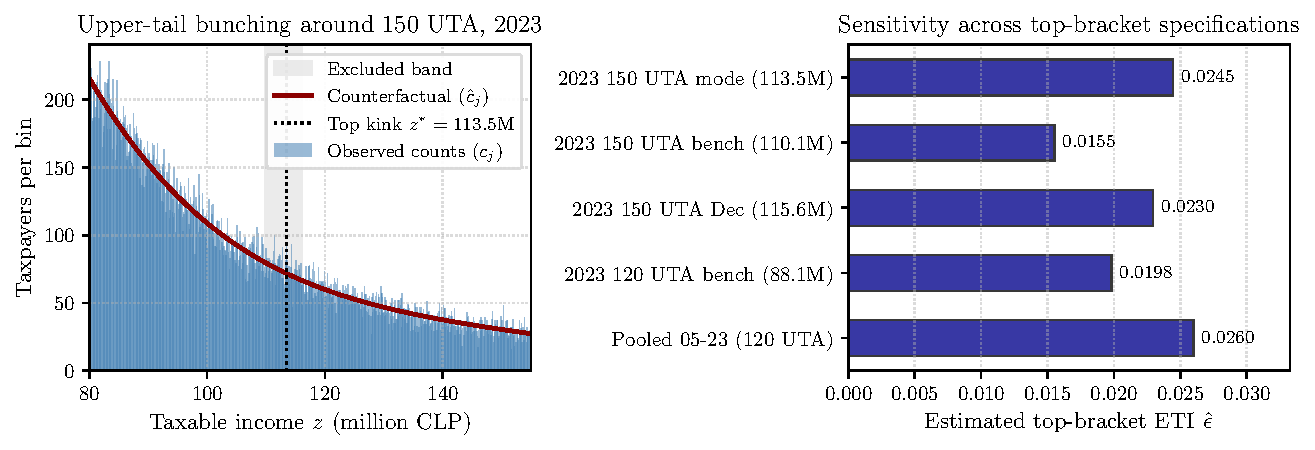
\includegraphics[width=\textwidth]{p3/p3_top_bunching.pdf}
\caption{Top-bracket bunching estimation on \texttt{synthetic\_bunch\_counts.csv}. Left panel: observed 2023 counts and fourth-degree Chetty-reweighted counterfactual over $[\$80\text{M}, \$155\text{M}]$ CLP with excluded region $[\$110\text{M}, \$116\text{M})$ CLP around the $150\text{ UTA}$ mode ($z^* = \$113.50\text{M}$ CLP). Right panel: comparison of estimated top-bracket elasticities $\hat{\epsilon}$ across upper-tail cutoff definitions and multi-year pooling.}
\label{fig:p3_bunching}
\end{figure}

\begin{table}[htbp]
\centering
\caption{Calibrated top-bracket $|\mathrm{MVPF}|$ across Problem Set 1 Pareto parameters ($\hat{\alpha}$) and bunching elasticities ($\hat{\epsilon}$)}
\label{tab:p3_mvpf}
\small
\begin{adjustbox}{max width=\textwidth}
\begin{tabular}{lrrrrrrrr}
\toprule
Pareto tail specification (PS1) & $\hat{\epsilon}$ & $\hat{\alpha}$ & $\hat{\epsilon}\hat{\alpha}$ & Offset ($\tau_0$) & $|\mathrm{MVPF}(\tau_0)|$ & $|\mathrm{MVPF}(\tau_1)|$ & $|\mathrm{MVPF}(\bar{\tau})|$ & $\overline{|\mathrm{MVPF}|}_{\mathrm{exact}}$ \\
\midrule
PS1 Vermeulen MLE ($w_{\min}=380\text{M}$, $\hat{\alpha}=1.859$) & 0.0245 & 1.859 & 0.0455 & 3.03\% & 1.0313 & 1.0251 & 1.0280 & 1.0281 \\
PS1 SII Top Bracket ($>310\text{ UTA}$, $\hat{\alpha}=2.085$) & 0.0245 & 2.085 & 0.0510 & 3.40\% & 1.0352 & 1.0282 & 1.0316 & 1.0316 \\
PS1 Gabaix--Ibragimov Reg ($w_{\min}=380\text{M}$, $\hat{\alpha}=2.135$) & 0.0245 & 2.135 & 0.0522 & 3.48\% & 1.0361 & 1.0289 & 1.0323 & 1.0324 \\
PS1 Vermeulen MLE ($w_{\min}=P99$, $\hat{\alpha}=2.531$) & 0.0245 & 2.531 & 0.0619 & 4.13\% & 1.0430 & 1.0345 & 1.0386 & 1.0386 \\
\midrule
PS1 Vermeulen MLE ($w_{\min}=380\text{M}$, $\hat{\alpha}=1.859$) & 0.0155 & 1.859 & 0.0288 & 1.92\% & 1.0196 & 1.0158 & 1.0176 & 1.0176 \\
PS1 SII Top Bracket ($>310\text{ UTA}$, $\hat{\alpha}=2.085$) & 0.0155 & 2.085 & 0.0324 & 2.16\% & 1.0220 & 1.0177 & 1.0198 & 1.0198 \\
PS1 Gabaix--Ibragimov Reg ($w_{\min}=380\text{M}$, $\hat{\alpha}=2.135$) & 0.0155 & 2.135 & 0.0331 & 2.21\% & 1.0226 & 1.0182 & 1.0203 & 1.0203 \\
PS1 Vermeulen MLE ($w_{\min}=P99$, $\hat{\alpha}=2.531$) & 0.0155 & 2.531 & 0.0393 & 2.62\% & 1.0269 & 1.0216 & 1.0241 & 1.0242 \\
\midrule
PS1 Vermeulen MLE ($w_{\min}=380\text{M}$, $\hat{\alpha}=1.859$) & 0.0260 & 1.859 & 0.0483 & 3.22\% & 1.0333 & 1.0267 & 1.0298 & 1.0299 \\
PS1 SII Top Bracket ($>310\text{ UTA}$, $\hat{\alpha}=2.085$) & 0.0260 & 2.085 & 0.0542 & 3.61\% & 1.0375 & 1.0300 & 1.0336 & 1.0336 \\
PS1 Gabaix--Ibragimov Reg ($w_{\min}=380\text{M}$, $\hat{\alpha}=2.135$) & 0.0260 & 2.135 & 0.0555 & 3.70\% & 1.0384 & 1.0308 & 1.0344 & 1.0345 \\
PS1 Vermeulen MLE ($w_{\min}=P99$, $\hat{\alpha}=2.531$) & 0.0260 & 2.531 & 0.0657 & 4.38\% & 1.0458 & 1.0367 & 1.0411 & 1.0411 \\
\midrule
PS1 Vermeulen MLE ($w_{\min}=380\text{M}$, $\hat{\alpha}=1.859$) & 0.2570 & 1.859 & 0.4778 & 31.85\% & 1.4674 & 1.3464 & 1.4019 & 1.4035 \\
PS1 SII Top Bracket ($>310\text{ UTA}$, $\hat{\alpha}=2.085$) & 0.2570 & 2.085 & 0.5358 & 35.72\% & 1.5558 & 1.4055 & 1.4739 & 1.4761 \\
PS1 Gabaix--Ibragimov Reg ($w_{\min}=380\text{M}$, $\hat{\alpha}=2.135$) & 0.2570 & 2.135 & 0.5487 & 36.58\% & 1.5768 & 1.4193 & 1.4908 & 1.4932 \\
PS1 Vermeulen MLE ($w_{\min}=P99$, $\hat{\alpha}=2.531$) & 0.2570 & 2.531 & 0.6505 & 43.36\% & 1.7657 & 1.5391 & 1.6401 & 1.6442 \\
\bottomrule
\end{tabular}
\end{adjustbox}
\begin{minipage}{\textwidth}
\vspace{4pt}
\footnotesize\textit{Note:} Local MVPFs evaluated at $\tau_0 = 0.40$, $\tau_1 = 0.35$, and midpoint $\bar{\tau} = (\tau_0+\tau_1)/2 = 0.375$, alongside the exact analytical integral $\overline{|\mathrm{MVPF}|}_{\mathrm{exact}}$ over $[0.35, 0.40]$. ``Offset ($\tau_0$)'' denotes the behavioral revenue share $-\Delta R^B / \Delta R^M = \frac{\tau_0}{1-\tau_0}\hat{\epsilon}\hat{\alpha}$ at $\tau_0 = 0.40$. The four groups of rows correspond to: (1) 2023 top-kink bunching at the 150 UTA empirical mode ($\hat{\epsilon}=0.0245$), (2) 2023 150 UTA statutory benchmark ($\hat{\epsilon}=0.0155$), (3) pooled 2005--2023 120 UTA bunching ($\hat{\epsilon}=0.0260$), and (4) the synthetic first-kink upper-bound benchmark ($\hat{\epsilon}=0.2570$).
\end{minipage}
\end{table}


Table~\ref{tab:p3_mvpf} and Figure~\ref{fig:p3_mvpf} report the calibrated values\footnote{\texttt{code: source/bunching/mvpf.py:L105}} of $|\mathrm{MVPF}(\tau_0)|$ at $\tau_0 = 0.40$, $|\mathrm{MVPF}(\tau_1)|$ at $\tau_1 = 0.35$, the midpoint approximation $|\mathrm{MVPF}(\bar{\tau})|$ at $\bar{\tau} = 0.375$, and the exact analytical average $\overline{|\mathrm{MVPF}|}_{\mathrm{exact}}$ from~\eqref{eq:p3_mvpf_exact}:
\begin{itemize}
    \item \textbf{Baseline top-bracket bunching regime ($\hat{\epsilon}_{\mathrm{top}} = 0.0245$):} Paired with the Problem Set~1 baseline Pareto index $\hat{\alpha}_{\mathrm{MLE}} = 1.859$, the product $\hat{\epsilon}\hat{\alpha} = 0.0455$ implies that behavioral responses offset only $3.03\%$ of the mechanical revenue change at $\tau_0 = 0.40$ and $2.45\%$ at $\tau_1 = 0.35$. Consequently, $|\mathrm{MVPF}(0.40)| = 1.0313$, $|\mathrm{MVPF}(0.35)| = 1.0251$, the midpoint estimate is $|\mathrm{MVPF}(0.375)| = 1.0280$, and the exact integral is $\overline{|\mathrm{MVPF}|}_{\mathrm{exact}} = 1.0281$. Across all four PS1 Pareto estimates ($\hat{\alpha} \in [1.859,\, 2.531]$) and all three upper-tail bunching estimates ($\hat{\epsilon} \in [0.0155,\, 0.0260]$), the average MVPF stays tightly bounded within $[1.0176,\, 1.0411]$, and the midpoint approximation matches the exact integral to four decimal places.
    \item \textbf{Upper-bound ETI sensitivity ($\hat{\epsilon} = 0.2570$):} If top-bracket taxpayers responded with the much larger elasticity observed at the first kink ($\hat{\epsilon} = 0.2570$), the behavioral revenue offset at $\tau_0 = 0.40$ would rise to $31.85\%$ under $\hat{\alpha}_{\mathrm{MLE}} = 1.859$ (and $43.36\%$ under $\hat{\alpha}_{\mathrm{MLE},P99} = 2.531$), pushing the average MVPF to $\overline{|\mathrm{MVPF}|}_{\mathrm{exact}} = 1.4035$ (and up to $1.6442$ at the P99 tail index). Even under this upper-bound elasticity, $\tau_0 = 0.40$ lies well below the revenue-maximizing Laffer peak $\tau^{\mathrm{Laffer}} = (1 + \hat{\epsilon}\hat{\alpha})^{-1} \in [0.606,\, 0.677]$.
\end{itemize}

\begin{figure}[htbp]
\centering
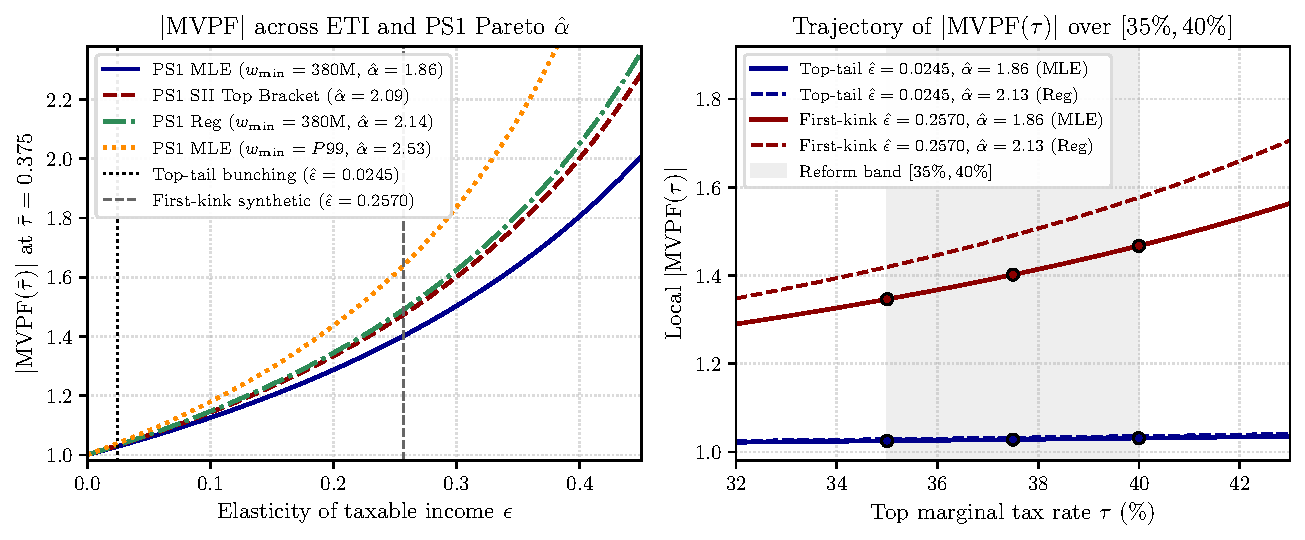
\includegraphics[width=\textwidth]{p3/p3_mvpf_calibration.pdf}
\caption{Calibrated top-bracket $|\mathrm{MVPF}|$ across Problem Set~1 Pareto parameters and bunching elasticities. Left panel: $|\mathrm{MVPF}(\bar{\tau})|$ at $\bar{\tau} = 0.375$ as a function of $\epsilon$ for four PS1 Pareto indices $\hat{\alpha}$, marking the 2023 top-tail bunching estimate ($\hat{\epsilon} = 0.0245$) and the synthetic first-kink reference ($\hat{\epsilon} = 0.2570$). Right panel: trajectory of local $|\mathrm{MVPF}(\tau)|$ across the $[35\%, 40\%]$ reform window.}
\label{fig:p3_mvpf}
\end{figure}

\subsection*{(iii) Policy brief: Evaluating a $40\% \to 35\%$ top marginal rate cut}

A reduction in Chile's top personal income tax rate from $40\%$ to $35\%$ transfers disposable income to taxpayers in the highest bracket at the cost of foregone public revenue. Calibrating the sufficient-statistic MVPF model with our Problem Set~1 Pareto tail indices ($\hat{\alpha} \in [1.859,\, 2.531]$) and upper-bracket bunching elasticities ($\hat{\epsilon}_{\mathrm{top}} \in [0.0155,\, 0.0260]$, baseline $0.0245$) yields an average $|\mathrm{MVPF}|$ of \textbf{1.028 to 1.039} (and \textbf{1.404 to 1.644} under the first-kink upper-bound elasticity $\hat{\epsilon} = 0.2570$). Under the baseline empirical top-tail response, cutting the top rate by $5$ percentage points generates a behavioral revenue recovery of less than $3\%$--$4\%$ of the mechanical loss: every $\$1.00$ of private tax relief delivered to top-bracket earners costs the public budget roughly $\$0.97$ in net revenue.


Interpreting Equations~\eqref{eq:p3_mech}--\eqref{eq:p3_mvpf} as guideposts for Chilean fiscal policy requires scrutinizing four structural assumptions:
\begin{enumerate}
    \item \textbf{Type-I Pareto tail ($\alpha$ constant above $z^*$):} As verified in Problem Set~1, Chile's upper income and wealth distribution is well approximated by a power law ($\hat{\alpha} \approx 1.86$--$2.14$). However, because top wealth is substantially more concentrated than salaried wage income, applying a wealth-based $\hat{\alpha}_{\mathrm{MLE}} = 1.859$ (thick tail) alongside $\hat{\alpha}_{\mathrm{Reg}} = 2.135$ or $\hat{\alpha}_{\mathrm{SII}} = 2.085$ provides a conservative upper bound on the Pareto hazard ratio $\bar{y}/(\bar{y}-z^*)$.
    \item \textbf{Quasilinear isoelastic utility and local bunching identification:} The model rules out income effects and assumes that the local bunching elasticity at the bracket cutoff equals the structural elasticity governing responses across the entire upper tail. In practice, bunching in \texttt{synthetic\_bunch\_counts.csv} is measured on formal wage earners below $\$159.9\text{M}$ CLP (whereas the post-2020 $40\%$ bracket begins at $310\text{ UTA} \approx \$227.5\text{M}$ CLP) and is attenuated by contractual rigidities and adjustment costs ($\phi > 0$, Section~2(i)).
    \item \textbf{Absence of cross-base fiscal externalities:} Equation~\eqref{eq:p3_mvpf} assumes that declared personal taxable income $z$ is the sole tax base affected by $\tau$. In Chile's semi-integrated corporate tax system, top-One-Percent taxpayers derive the vast majority of their income from accrued capital and retained corporate profits rather than wages \parencite{gutierrezNoExemption}. Lowering the personal top rate from $40\%$ to $35\%$ primarily alters the timing of dividend distributions and income shifting between corporate and personal bases rather than expanding real labor supply.
    \item \textbf{Unitary social welfare weights ($g_{\mathrm{top}} = 1$):} Reporting $|\mathrm{MVPF}| \approx 1.03$ equates the social value of an additional peso in the hands of a top-$0.1\%$ earner with an additional peso of public revenue. In standard optimal-taxation frameworks with diminishing marginal utility of consumption, the social marginal welfare weight on the top bracket is close to zero ($g_{\mathrm{top}} \approx 0$), implying a welfare-weighted MVPF of $g_{\mathrm{top}}\,|\mathrm{MVPF}| \ll 1$.
\end{enumerate}

\textbf{We recommend rejecting the proposed $40\% \to 35\%$ reduction in the top marginal rate.} First, the reform is fiscally costly and far from self-financing: across every calibrated $(\hat{\epsilon}, \hat{\alpha})$ pair in Table~\ref{tab:p3_mvpf}, the current $40\%$ rate sits well below the Laffer peak ($\tau^{\mathrm{Laffer}} \ge 60.6\%$), and under upper-tail wage bunching ($\hat{\epsilon}_{\mathrm{top}} \approx 0.0245$) more than $96\%$ of the mechanical tax cut translates directly into permanent revenue loss. Second, the reform is sharply regressive: it concentrates tax relief entirely on the top $<0.2\%$ of adults (those above $310\text{ UTA}$) in a country where top earners already face low effective tax rates ($11\%$--$16\%$) due to corporate profit retention \parencite{gutierrezNoExemption}. Third, even if top-end reporting elasticities exceed salaried bunching estimates ($\hat{\epsilon} \approx 0.26$), that responsiveness reflects tax avoidance and inter-base shifting through holding companies rather than real productive effort; the appropriate policy response is to tighten anti-avoidance rules and harmonize capital-income taxation rather than lowering the statutory top rate.